\subsection{MOS gate}\label{gate_dimensioning}
As the continuous down-scaling of the device size has lead to very thin gate oxides, the leakage current that can flow from the channel to the gate comes into the order of the subthreshold leakage current and the gate cannot be considered as an ideally insulated electrode anymore.
This affects the circuit functionality and increases the standby power consumption due to the static gate current.
For dynamic logic concepts the gate leakage drastically reduces the maximum clock cycle time\footnote{N. Wang, Digital MOS Integrated Circuits, Prentice-Hall, Englewood Cliffs, NJ, 1989}.
Two tunneling mechanisms are responsible for the gate leakage, Fowler-Nordheim tunneling and direct tunneling\footnote{A. Schenk and G. Heiser, "Modeling and Simulation of Tunneling through Ultra-Thin Gate Dielectrics"J.Appl.Phys., vol. 81, no. 12, pp. 7900, 1997}.
The gate leakage increases exponentially as the oxide thickness is reduced.
This limits the down-scaling of the oxide thickness to about 1.5-2 nm when looking at the total standby power consumption of a chip\footnote{Y. Taur, "The Incredible Shrinking Transistor," IEEE Spectrum, pp. 25-29, July 1999.}.
To further decrease the effective oxide thickness alternative high dielectric constant materials can be used\footnote{S. Thompson, P. Packan, and M. Bohr, "MOS Scaling: Transistor Challenges for the 21st Century," Intel Technology Journal, vol. Q3, 1998}.
On the other hand, a thin gate oxide reduces the short-channel effect and improves the driving capabilities of a MOS transistor.
However, a tradeoff between this benefit and the gate leakage is necessary.\\

With $1 \mu m$ we don't have to worry about this leakage yet because our gate oxide thickness is too high for these effects to actually become a problem, but we want to do our home work already in preparation of scale-down and also for curiosity.

We for now just use 40 nm. That's still doable with a precision high enough when using dry oxidation and a temperature of 1000\degree Celsius.

\subsubsection{Subthreshold leakage}

The sub-threshold leakage current can be calculated with\footnote{\url{http://ecee.colorado.edu/\~bart/book/book/chapter3/ch3_4.htm\#3_4_2}}
\begin{equation}
I_{sub}
=
I_0
\cdot
\left(1-\exp\left(-\frac{V_{ds}}{V_{th}}\right)\right)
\cdot
\exp\left(\frac{V_{gs}-V_{T}}{n \cdot V_{th}}\right)
\end{equation}

where
\begin{equation}
I_0 = \frac{W}{L} \mu_0 V_{th}^2 \sqrt{\frac{N_A \cdot q \cdot \epsilon_{Si}}{2 \cdot \phi_{sub}}}
\end{equation}
$V_{th}=26mV$ is the thermal voltage, $V_T$ is the threshold voltage, $V_{ds}$ and $V_{gs}$ are the drain-to-source and gate-to-source voltages respectively.
W and L are the effective transistor width and length, respectively. $C_{ox}$ is the gate oxide capacitance, $\mu_0$ is the carrier mobility and $n=1+\frac{C_{dep}}{C_{ox}}$ is the subthreshold swing coefficient.

First of all, lets say $W=L$ which leads to a square:
\begin{equation}
I_0 = \mu_0 V_{th}^2 \sqrt{\frac{N_A \cdot q \cdot \epsilon_{Si}}{2 \cdot \phi_{sub}}}
\end{equation}

With
\begin{itemize}
\item $\epsilon_0 = 8.85 \cdot 10^{-14}\frac{F}{cm}. $ is the electric permittivity in vacuum
\item $\epsilon_{ox} =3.9 \cdot \epsilon_0$ is the relative permittivity of silicon dioxide
\item $\epsilon_{Si} =11.68 \cdot \epsilon_0$ is the relative permittivity of silicon
\end{itemize}

The carrier mobility $ \mu_0$ can be calculated with\footnote{\url{https://ecee.colorado.edu/\~bart/book/book/chapter2/ch2_7.htm\#2_7_2}}
\begin{equation}
 \mu(N) =  \mu_{min} + \frac{ \mu_{max}- \mu_{min}}{1+\left(\frac{N}{N_r}\right)^\alpha}
\end{equation}
using the fitting parameters from \autoref{fitting_parameters_mobility}

\begin{table}[H]
	\centering
	\begin{tabular}{|c|c|c|c|}
		\hline
		{} &
		\textbf{Arsenic} &	
		\textbf{Phosphorus} &
		\textbf{Boron} \\
		\hline
		$\mu_{min} [\frac{cm^2}{Vs}]$ &
		52.2 &
		68.5 &		
		44.9 \\
		\hline
		$\mu_{max} [\frac{cm^2}{Vs}]$ &
		1417 &
		1414 &
		470.5 \\
		\hline
		$N_r [\frac{1}{cm^3}]$ &
		$9.68 \cdot 10^{16}$ &
		$9.20 \cdot 10^{16}$ &
		$2.23 \cdot 10^{17}$ \\
		\hline
		$\alpha$ &
		0.68 &
		0.711 &
		0.719 \\
		\hline
	\end{tabular}
	\caption{Parameters for calculation of the mobility as a function of the doping density}
	\label{fitting_parameters_mobility}
\end{table}

We can now plot multiple leakages for N- and P-channel transistors with a gate oxide thickness\footnote{See simulation/gate.wxmx} wit a surface concentration of $1e16\frac{1}{cm^3}$
\begin{figure}[H]
	\centering
	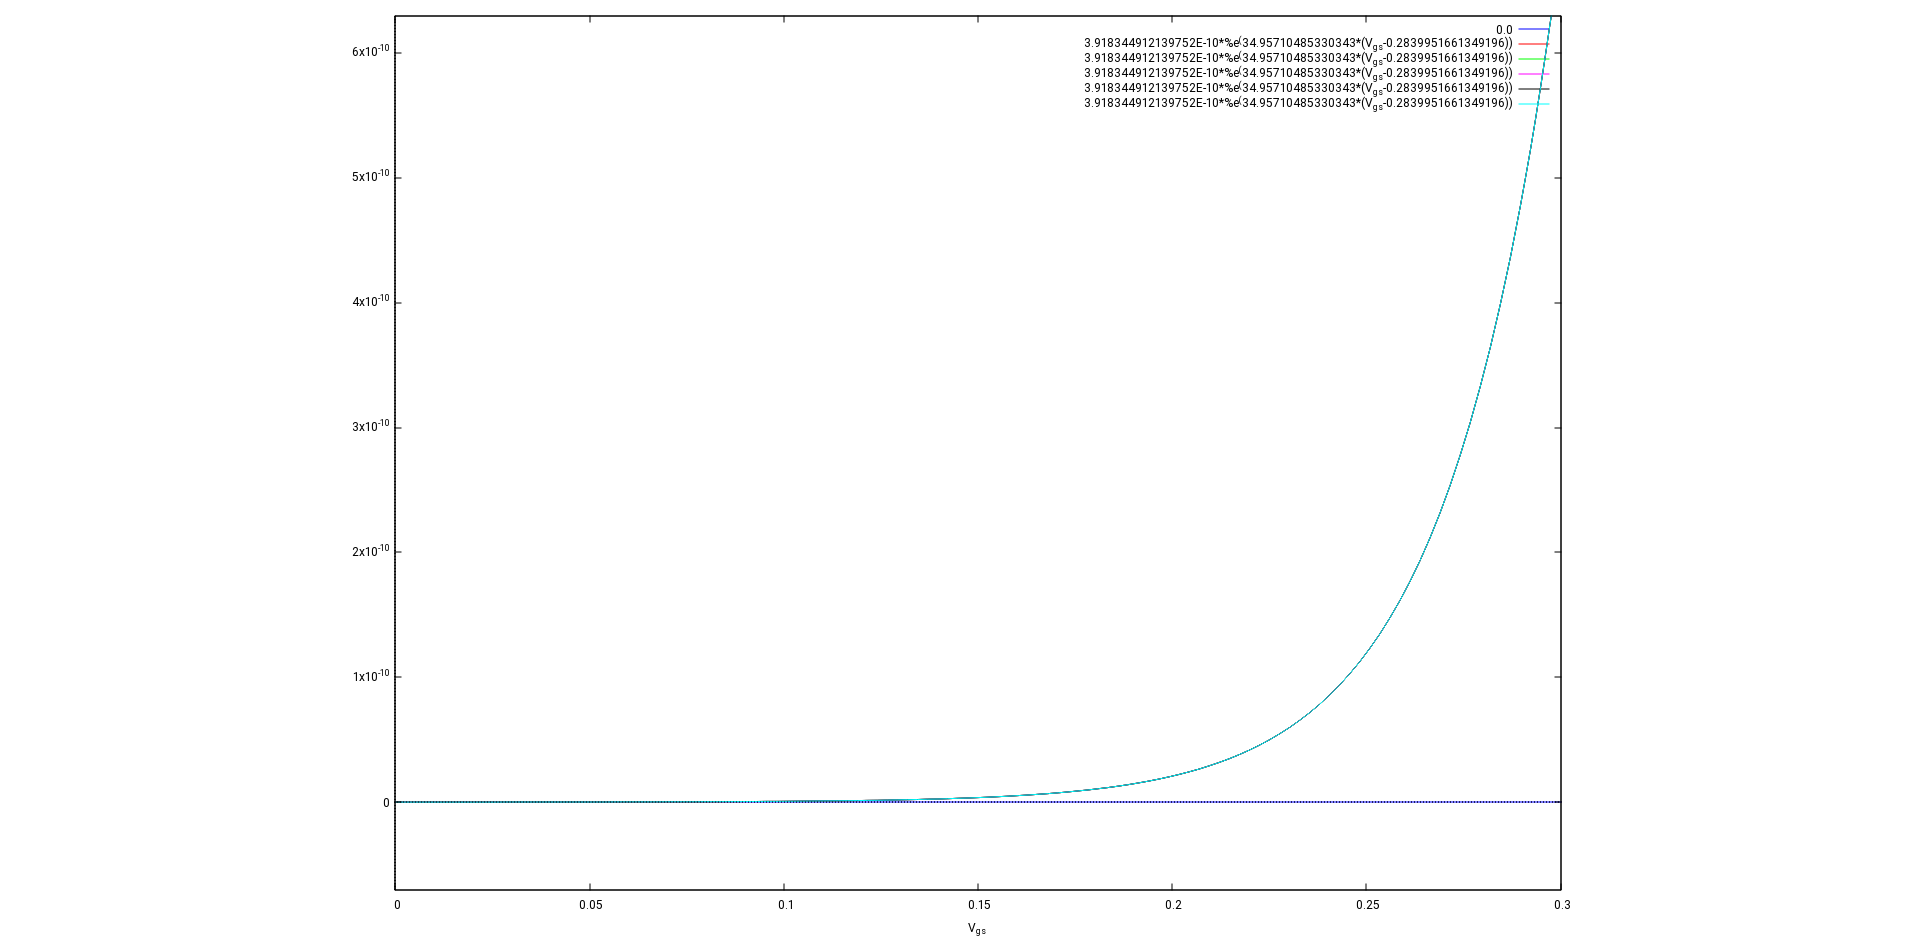
\includegraphics[width=\textwidth]{subthreshold_leagage.png}
	\caption{Subthreshold leakage plot(in Ampere)}
	\label{leagage_currents}
\end{figure}
In \autoref{leagage_currents} we see that with our gate oxide thickness this is really no problem, as we had expected.
From 0V up to 5V and further there is basically no leakage on the gate from the sub threshold current with $V_{Tn} \approx 0.28V$ and $V_{Tp} \approx -0.29V$.
That's good enough, as we will see in \autoref{nmos_dimensioning} and \autoref{pmos_dimensioning}.
There is actually a reduction of current when reaching the threshold because of the inversion of the capacity in the depletion zone\footnote{\url{https://people.eecs.berkeley.edu/~hu/Chenming-Hu_ch5.pdf}}, but I didn't include this into the calculation, because "TL;DR".
It's a TODO for release 2.1 of this process which will go sub $1 \mu m$

\subsubsection{Gate tunneling current}

The tunneling of electrons (or holes) from the bulk and source/drain overlap region through the gate oxide potential barrier into the gate (or vice-versa) is referred as gate oxide tunneling current.
This phenomenon is related with the MOS capacitance concept.
There are three major gate leakage mechanisms in a MOS structure.
The first one is the electron conduction-band tunneling (ECB), where electrons tunneling from conduction band of the substrate to the conduction band of the gate (or vice versa).
The second one is the electron valence-band tunneling (EVB). In this case, electrons tunneling from the valence band of the substrate to the conduct band of the gate.
The last one is known as hole valence-band (HVB) tunneling, where holes tunneling from the valence band of the substrate to the valence band of the gate (or vice- versa)

Each mechanism is dominant or important in different regions of operation for NMOS and PMOS transistors. For each mechanism, gate leakage current can be modeled by
\begin{equation}
I = W \cdot L \cdot A \cdot \left(\frac{V_{ox}}{t_{ox}}\right)^2\exp\left(\frac{-B\left(1-\left(1-\frac{V_{ox}}{\phi_{ox}}\right)^{\frac{3}{2}}\right)}{\frac{T_{ox}}{t_{ox}}}\right)
\end{equation}
